%----------------------------------------------------------------------------   
\chapter{Architektúra}
%----------------------------------------------------------------------------

A Kubernetes architektúra tervezése során a fő szempont az volt, hogy teljes
mértékben úgy nézzen ki kívülről, mintha egy szimpla rtpengine lenne. De 
mögötte egy mikroszolgáltatásokból álló alkalmazás legyen, mely képes
az benne rejlő rtpengine-t megfelelően konfigurálni.

Ezt a fürtöt a BME által szolgáltatott szervereken építettem ki, mi szám szerint
4 szervert tartalmaz melyek az alábbi elrendezésben vannak összekötve.

\begin{figure}[!ht]
	\centering
	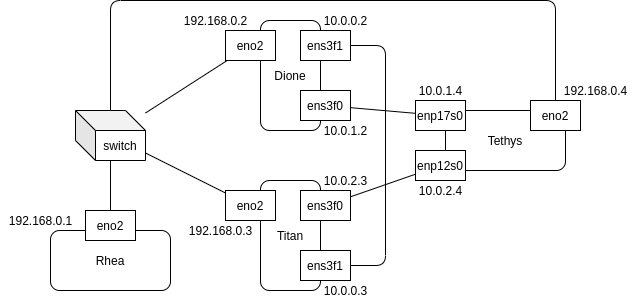
\includegraphics[width=1\textwidth, keepaspectratio]{figures/servers.png}
	\caption{Szerverek összeköttetése}
	\label{fig:HVSpaces}
\end{figure}

Az ábrán szereplő szervereket kettő részre lehet szétbontani, ahol az egyik
konkréten a Kubernetes fürt a másik pedig a forgalom generálására használatos.
Az előbbibe tartozik a Rhea, mint mester csomópont és dolgozó csomópontok közé 
a Dione és a Titan. Majd értelemszerűen az utóbbiba tartozik a Tethys. 

A szerverek között a kapcsolatot a vonalakkal jeleztem, melyek, mint látszik
sok esetben direkt összeköttetésben vannak egymással. Ez azért van, mert ezek
az interfészek 40 gigabitesek és az egyetemen nem állt rendelkezésre ilyen 
sebességű switch. Ezáltal a Kubernetes fürt telepítése során különös figyelmet
kellett szentelni annak, hogy ezek az interfészek helyesen legyenek felkonfigurálva.

De, mint látszik a hálózatban szerepel egy switch, amibe az eno2 interfészek vannak
becsatlakoztatva. Ezek az interfészek 1 gigabites sebességgel rendelkeznek, amik
a sok nagy sebességű forgalmat nem képes kiszolgálni, viszont még így is hasznosak
a hálózat szempontjából. Mivel a telepített Kubernetes fürt vezérlő- és adatsíkja
ezen a két összeköttetésen osztozik. Szóval a lassabb interfészeken kommunikál az
API szerver és a kubelet, míg a kube-proxy a nagy sebességű hálózati kártyákat 
használja. Így lehetett egy olyan magas határt szabni a lehetséges forgalom
sebességének, amibe nehéz beleütközni. 

Ahhoz, hogy az előzőleg leírt hálózat elkülönítés működjön a Kuberspray programot 
használtam, mert ennél könnyedén lehetett a telepítés során kettő különböző interfészt
beállítani. A kuberspray programmal Kubernetes fürtöket lehet telepíteni szimplán
szerverekre. A különlegessége az, hogy Ansible-t használ erre a célra. Szóval elég
a mester szerver számára lehetővé tenni, hogy működjön az ssh a többi szerverrel és
egyetlen konfigurációs fájl indításával képes minden szükséges szoftvert feltelepíteni
és azokat beállítani. Az Ansible-l nagyjából bármilyen folyamatot lehet automatizálni a
szerverek között. 

\section{Kubernetes architektúra}

A címben említett architektúra írja le, hogy a fürtön belül milyen Kubernetes
erőforrások találhatóak meg és azok, hogyan vannak egymással összekötve. A következő
ábrát kifejtve lehet ezt legjobban elmagyarázni. Fontos megjegyezni, hogy erre 
a rengeteg átalakításra azért van szükség, mert a kamailio nem legfrissebb
stabil verziója nem tud WebSocket-n keresztül vezérlőcsomagokat küldeni és az rtpengine-nek
az a verziója, amivel a redis-t ilyen módon lehet használni nem támogatja szintúgy
a WebSocket-t.

\begin{figure}[!ht]
	\centering
	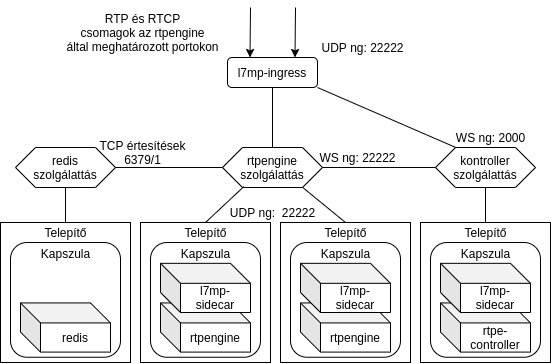
\includegraphics[width=1\textwidth, keepaspectratio]{figures/cluster.png}
	\caption{Fürt felépítése}
	\label{fig:HVSpaces}
\end{figure}

\subsection{Ingress}

Mint látszik a hálózatba való belépés az l7mp-ingress kapun történik, ahol kezdetben
statikusan konfigurálva van egy figyelő, ami a dolgozó csomópont 22222 UDP portján
vár minden az rtpengine-nek szánt vezérlőüzenetet. De látszik, hogy a kontroller szolgáltatás
a 2000-s WebSocket porton várja az üzeneteket. Ezért az l7mp-ingress ezen figyelőjének 
tudnia kell UDP csomagokat WebSocket-re átalakítani. Ez az l7mp-nek köszönhetően nagyon
egyszerűen megvalósítható volt ugyanis, elég csak egy UDP figyelőt létrehozni majd azt 
egy WebSocket fürthöz irányítani, aminek a végpontja a kontroller szolgáltatás. 


\subsection{Kontroller}
A kontroller a beérkező vezérlőüzeneteket automatikusan továbbítja az rtpengine 
szolgáltatásnak WebSocket-n keresztül. Mielőtt fojtatnám azzal, hogy a kontroller milyen 
feladatokat lát el fontos kifejteni a WebSocket protokoll szükségességét ebben az esetben.
Mivel minden WebSocket-nek  csomag rendelkezik egy HTTP-hez hasonló fejléccel így
lehet egyéni információkat küldeni fejlécekben. Ez az információ ebben az esetben a híváshoz
tartozó  két azonosítót jelent. Az egyik a hívásazonosító míg a másik a hívásban résztvevő
fél forrásazonosítója. Mivel ez a kettő információ fog szerepelni minden csomagban így elérhető az,
hogy a vezérlő üzenetek mindig ugyanahhoz a kapszulához jussanak el. Így elkerülhető az
az eset, hogy mondjuk egy answer és egy offer üzenet kettő különböző rtpengine kapszulához
jusson el. Így a kontroller pótkocsijában kettő figyelőnek kell szerepelnie, az egyik
az amin az l7mp-ingress-től várja a vezérlőüzeneteket és a másik, amin a helyi hálózatról
várja azokat az üzeneteket, amiket el kell küldenie az rtpengine felé. 

De visszatérve arra, hogy a kontrollerre miért is van szükség. A kontrollernek két fő feladata
van. Az első, hogy a hívásokhoz szükséges CRD-ket létrehozza és törölje, így az operátor tudni fogja,
hogy milyen beállításokat kell alkalmaznia az l7mp proxy pótkocsikban. Aztán van a másik feladata,
amivel a kimenő üzeneteket kell átírni annak megfelelően, hogy a dolgozó csomópont
címe legyen benne és ne 127.0.0.1, mert az rtpengine mindig ezt a címet fogja beletenni
a módosított SDP üzenetekbe. 

\subsection{rtpengine}

Az rtpengine ebben az esetben teljesen ugyanazt a funkciót látja el, mint egy normális hívás
esetében azzal a különbséggel, hogy képes redundánsan működni. Szóval, ha az egyiken létrejön
egy hívás, akkor az létezni fog a másikon is és képes rögtön kezelni a beérkező forgalmat. Ezt
oly módon teszi, hogy minden híváshoz létrehoz egy rekordot a Redis adatbázisban, ami 
keyspace-ket (kulcshelyeket) használ. Azért van szükség arra, hogy kulcshely tábla legyen
használva az adatbázisban, mert erre fellehet iratkozni. Szóval a két rtpengine kapszula
feliratkozik ugyanarra a kulcshelyre, ahova mind a két kapszula fogja írni a beérkező hívásaikat.
Így, ha az egyik kapott egy hívást az létrehoz egy rekordot az adott kulcshelyen, amiről a 
Redis értesíti a másik kapszulát és elküldni annak ezeket az információkat, ami majd létrehozza
az adott hívást és kinyitja az hozzá szükséges portokat.  

De ez a funkció ebben a formában nem szerepel az rtpengine-ben. A hivatalos verzióban csak úgy 
működik, ha minden rtpengine példány látja egymást a hálózaton és már létrejöttükkor tudják
egymás címét és, hogy melyik példány melyik kulcshelyet használja. Ez Kubernetes hálózatban
nem túl szerencsés megoldás, mivel a kapszulák bármikor törlődhetnek és más címmel jöhetnek 
létre. Ezért kellett találni egy megoldást, amit egy bizony Oded Arbell pull request-je (ajánlása)
jelentett. Ugyanis szerette volna, ha lehet skálázni az rtpengine példányokat anélkül, hogy 
tudnánk a létező többinek a címét is. Ezt majdnem teljesen jól megoldotta, viszont egy olyan 
problémába ütközött, hogy SRTP esetén nem minden hívást képes felépíteni az újonnan létrejött
rtpengine. Így nem olvasztották be a fő kódbázisba, ezért nem tudom a hivatalos rtpengine-t használni.

Viszont itt még nem oldódott meg teljesen a probléma, ugyanis ez a verziója az rtpengine-nek csak
skálázásra működött így, ha kettő példány fut egymás mellett, nevezzük őket \textbf{A}, 
\textbf{B}-nek. Akkor, ha \textbf{A}-hoz beérkezik egy hívás, erről értesül \textbf{B}, viszont nem
nyitja ki hozzá a megfelelő portokat. Így, ha bármi történik \textbf{A}-val \textbf{B} nem tudja
fogadni a hozzá beérkező forgalmat. Ennek a kiküszöbölése gyanánt egy kicsit módosítanom 
kell az rtpengine kódján, hogy mikor frissítés történik az adatbázisból, akkor portokat is nyisson ki.
Ez egy elfogadható megoldásnak lehet tartani átlag esetben, viszont a Kubernetes világában
ez a megoldás nem a legszebbek közé tartozik, mert nem követi a Kubernetes által diktált
irányokat. A szép megoldás az lenne, ha a \textbf{B} példányon csak akkor nyílnának ki ezek a 
portok, ha \textbf{A} biztosan megszűnt. Ezt a későbbiek során lehet javítani. \\

A pótkocsik még nagyon fontosak ennél a résznél. Mert egyrészt van egy figyelő, ami a kontroll
üzenetekre figyel és végzi az átalakítást WebSocket-ről UDP-re és van kettő másik, amik 
az RTP és RTCP üzeneteket fogják kezelni. Legegyszerűbben szemléltetni és kifejteni ezt is egy 
ábra segítségével lehet. 



 